    %LLPStartPreview para rodar o pdf com mudancas automaticas

\documentclass[12pt, a4paper]{article}
\usepackage{graphicx}
\usepackage{wrapfig}
\usepackage[utf8]{inputenc}
\usepackage[brazil]{babel} % Separacao de silabas em portugues
\usepackage{amsthm} % has proof
\usepackage{amsmath}
\usepackage{listings}
\usepackage{tcolorbox}
\usepackage {tikz}
\usepackage{hyperref}
\usepackage{float}
\usetikzlibrary {positioning}
\usetikzlibrary{arrows}
%\usepackage {xcolor}

\tikzset{edge/.style = {->,> = latex'}}

\graphicspath{
    {.} % document root dir
    {./img/}
}

\renewcommand\refname{Referências}
\newtheorem{theorem}{Teorema}[section]
\newtheorem{corollary}{Corolário}
\newtheorem{lemma}{Lema}

\title{O problema do carteiro chinês}
\author{Carlos Eduardo Ferreira\\Gabriel Fernandes de Oliveira}
\date{}

\begin{document}

\maketitle

\section{As sete pontes de Königsberg}

\begin{wrapfigure}{r}{0.5\textwidth} 
    \centering
    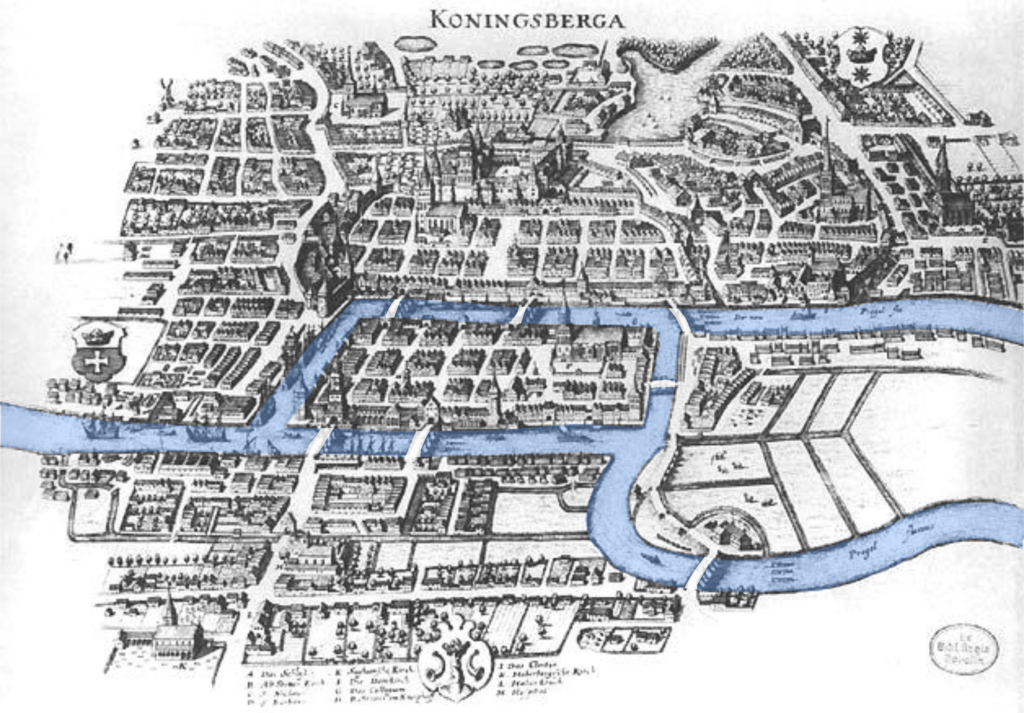
\includegraphics[width=0.5\textwidth]{konigsberg.png}
    \caption{Representação das sete pontes de Königsberg}
\end{wrapfigure}

O problema das sete pontes de Königsberg foi descrito e solucionado pelo matemático Leonhard Euler em 1736, o problema consistia em decidir se seria possível traçar no mapa de Königsberg um trajeto que percorresse cada uma de suas 7 pontes uma única vez, sem repetições.

Euler resolveu esse problema do seguinte modo: 
Primeiramente, ele identificou cada uma das massas de terra do mapa com as letras A, B, C e D.

Em seguida, ele definiu que um trajeto nesse mapa seria descrito por uma sequência dessas letras: por exemplo, "ACD" indicaria o trajeto que se inicia na massa de terra A, move-se para a massa de terra C, usando uma das pontes, e termina na massa D.

\begin{wrapfigure}{l}{0.5\textwidth} 
    \centering
    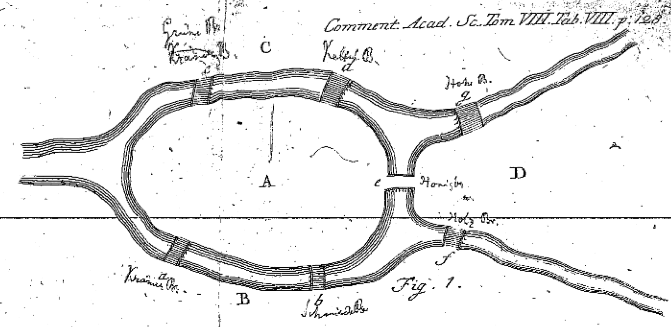
\includegraphics[width=0.5\textwidth]{konigsberg-euler.png}
    \caption{Representação de Euler}
	\label{konigsberg-euler}
\end{wrapfigure}

Euler então começou a definir algumas restrições, assumindo que o problema possuiria alguma solução:

Como o trajeto final deverá passar por todas as 7 pontes exatamente uma vez, isso implica que a sequência de letras que o representa deverá ter tamanho 8.

Além disso, como a massa de terra A possui 5 pontes, necessariamente a letra A aparecerá exatamente 3 vezes na sequência.
A massa B, C e D, no entanto possuem 3 pontes, portanto, suas letras correspondentes deverão aparecer apenas 2 vezes na sequência. 

Chegamos assim a um absurdo, pois inicialmente provamos que a sequência de letras que representa uma solução deveria ter tamanho 8 e depois chegamos que a mesma deveria ter tamanho 9.
Provando assim, por absurdo, que não existe um trajeto como o pedido no enunciado do problema.


Essa obserevação que, aos olhos de hoje, parece muito simples, teve um impacto profundo nas áreas da Matemática e Computação.
A modelagem de Euler, tratando as massas de terra e pontes de forma abstrata foi absoluatmente inovadora e é o embrião da área da teoria dos grafos.


Vamos definir como \textbf{passeio} em um grafo uma sequência finita não vazia $P = \{ v_0, v_1, \dots, v_k\}$, cujos termos são vértices $v_i$ tal que, para todo $i$, $0 \leq i < k$, os vértices $v_{i}$ e $v_{i+1}$ são ligados por uma aresta. 
Os vértices $v_0$ e $v_k$ são a origem e o término de $P$, respectivamente; e os vértices $v_1, v_2, \dots, v_{k-1}$ são chamados vértices internos de P. 

Uma \textbf{trilha} é um passeio sem arestas repetidas. 
Um \textbf{caminho} é um passeio sem vértices repetidos.
Definimos o comprimento de um passeio, denotado por $||P||$, como o número de arestas de $P$.

Um passeio é considerado \textbf{fechado} se sua origem e término são iguais.

Uma trilha fechada é um \textbf{circuito}.

Devido às contribuições de Euler ao problema descrito, chama-se \textbf{trilha euleriana} como uma trilha que passa por todas arestas de um grafo e \textbf{grafo euleriano} como um grafo que possui um circuito euleriana fechada.

Euler modelou essa área da cidade como um grafo, representado na figura \ref{konigsberg-graph}, tratando as pontes como arestas e as massas de terra como vértices.

A partir de tal modelagem e das definições feitas, o problema de Königsberg consiste, em definir se o grafo que representa a cidade possui ou não uma trilha euleriana. 


\begin{wrapfigure}{l}{0.25\textwidth}
    \centering
    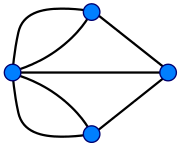
\includegraphics[width=0.25\textwidth]{konigsberg-graph.png}
    \caption{Modelagem de Königsberg como um grafo}
    \label{konigsberg-graph}
\end{wrapfigure}

Apesar de ter recebido grande parte do crédito histórico pelas suas implicações, Euler não provou que qualquer grafo conexo com vértices de grau par era euleriano, essa prova só foi publicada mais de cem anos depois, em 1873, por Carl Hierholzer \cite{hierholzer}, no que se tornou o conhecido Teorema de Euler.


\begin{theorem}[Teorema de Euler ou de Euler-Hierholzer]
    Um grafo é euleriano se, e somente se, é conexo e todos seus vértices possuem grau par.
    \label{euler}
\end{theorem}

Antes de mostrar a prova de tal teorema, primeiramente apresentaremos o seguinte lema:

Seja $\delta(G)$ o grau mínimo de um vértice pertencente a $G$.

\begin{lemma}
	\label{lema}
	Se $G$ é um grafo tal que $\delta(G) \geq 2$, então $G$ possui um circuito.
\end{lemma}

\begin{proof}
	Vamos assumir que um grafo qualquer $G = \{V, A\}$ não possui um caminho fechado. 
	Seja $P$ um caminho de comprimento maximal pertencente a $G$, denominamos $v$ um dos extremos de $P$. 
	Como $P$ é um caminho de comprimento maximal, é impossível, por definição, que $v$ possua uma aresta $vu$ que o ligue a um vértice $u$ não pertencente a $P$.
	
	Como, da premissa, todos vértices possuem grau maior ou igual a 2, isso implica que $v$ possuirá ao menos duas arestas que o ligam a vértices pertencentes a $P$.

	Porém, como $v$ é um vértice extremo de $P$, apenas uma dessas arestas pode pertencer ao caminho $P$. Isso implica que a outra aresta, digamos $vw$, não pertencente a $P$, implica na existência de um caminho fechado.

	Basta tomar o subcaminho entre os vértices $v$ e $w$ pertencente à $P$ juntamente com a aresta $vw$ que teremos um caminho fechado. Chegando assim em uma contradição.

	Demonstra-se assim que $G$ deverá possuir ao menos um caminho fechado dadas as condições do lema.
\end{proof}

Provado tal lema, podemos agora provar o teorema \ref{euler}:

\begin{proof}

Seja $G = \{V, E\}$ o grafo em questão.

($\Rightarrow$) Começamos provando que se um grafo é euleriano então todos seus vértices possuem grau par.

Seja $T$ um circuito euleriano, cuja existência é garantida já que $G$ é euleriano. Analisaremos o grau de um vértice qualquer $v$ de $G$.

Se $v$ não for um vértice extremo de $T$, então sempre que o mesmo aparecer em $T$ ele deverá ser precedido e sucedido de arestas. Indicando assim que $v$ deverá possuir um grau par.

Do contrário, se $v$ for o vértice extremo de $T$ ele necessariamente possui duas arestas, uma ligando-o ao segundo vértice do circuito, e outra o ligando ao penúltimo vértice de $T$. 
Além disso, cada aparição de $v$ como vértice interno de $T$ contabiliza mais duas arestas ao vértice em questão, de modo que $v$ possuirá um grau par ao final.

Sendo assim, se $G$ é euleriano, então todos seus vértices (extremos ou não) possuem grau par, como queriamos demonstrar.\newline

($\Leftarrow$) Agora, provaremos por indução no número de arestas de $G$ que se o grafo for conexo e se todos seus nós possuem grau par, então ele é euleriano.

O caso base da indução é quando não há arestas em $G$. 
O único grafo conexo que respeita tal condição é o grafo que possui apenas um vértice $v$.
Neste exemplo, $\{v\}$ é o circuito euleriano do grafo.

A hipótese de indução é que todo grafo simples, conexo, que possui até $k-1$ arestas e cujos vértices têm grau par é euleriano. 
Seja $G$ um grafo conexo, de vértices de grau par e que possua $k$ arestas, provaremos que ele também deverá ser euleriano.

Como $G$ é conexo, vale que $\delta(G) \geq 1$ e como todos nós de $G$ têm grau par, podemos afirmar que $\delta(G) \geq 2$. 
Sendo assim, pelo lema \ref{lema}, $G$ deverá possuir um circuito $C$.

Se $C$ possui todas arestas de $G$, então $C$ é um circuito euleriano do grafo, finalizando a prova.

Do contrário, aplicamos o seguinte procedimento para constuir um circuito euleriano $\mathcal{C}$ de $G$:

Retira-se de $G$ as arestas pertencentes a $C$, resultando assim em um grafo $G'$. 
Possivelmente $G'$ será desconexo, por isso definimos que $G'$ será a união de $k$ componenetes conexas $G'_1, G'_2, \dots, G'_k$ disjuntas entre si.

O grau dos vértices dessas componenentes $G'_i$ deverá ser par, já que, ao retirar todas as arestas de um circuito do grafo $G$, diminuimos o grau de um vértice qualquer $v$ em duas vezes o número de aparições do mesmo no circuito. mantendo assim a paridade dos graus. 

Além disso, cada componenete conexa de $G'$ possuirá uma quantidade de arestas menor do que $k$.
Portanto, pela hipótese da indução, cada uma dessas componentes deverá possuir um circuito euleriano próprio. 
Chamaremos de $C_i$ o circuito euleriano da componente $G'_i$.

Ao longo do algoritmo, os circuitos $C_i$ serão adicionados, um a um, ao circuito resultante $\mathcal{C}$. 
Definimos $\mathcal{T}$, como o conjunto dos circuitos eulerianos $C_i$ que ainda não fazem parte de $\mathcal{C}$. 
Inicialmente, $\mathcal{T}$ é igual ao conjunto $\{C_1, C_2, \dots, C_k\}$.


\[
	C = \{v, v_2, \dots, v_n, v\}
\]

Para cada vértice $u$ de $C$ devemos realizar as seguintes verificações:

\begin{tcolorbox}

Começamos adicionando $u$ ao circuito euleriano $\mathcal{C}$ que estamos construindo.

Enquanto houver um circuito euleriano $C_i$ pertencente a $\mathcal{T}$ do qual $u$ faz parte, fazemos o seguinte:


\begin{enumerate}
    \item Representamos $C_i$ como: 
    \[
        C_i = \{u, u_2, \dots, u_l, u\}
    \]

\item Adicionamos ao final de $\mathcal{C}$ o circuito $C_i$ como representado, exceto pelo primeiro vértice $u$. 

\item Removemos de $\mathcal{T}$ o circuito $C_i$, indicando que o mesmo já foi adicionado a $\mathcal{C}$.

\end{enumerate}

Repetem-se então as mesmas verificações para os próximos vértices de $C$.
\end{tcolorbox}


Ao final desse procedimento, o conjunto $\mathcal{T}$ deverá ser vazio, já que toda trilha $C_i$ possui pelo menos um vértice em $C$. Além disso, toda trilha $C_i$ deverá ter sido adicionada à $\mathcal{C}$ uma única vez, já que logo após adicionar uma trilha à $\mathcal{C}$ já a removiamos de $\mathcal{T}$, impedindo que ela fosse adicionada outra vez na trilha euleriana final.

Comprovado o passo da indução, finalizamos a prova do Teorema de Euler por indução.

\end{proof}

\begin{corollary}
    Um grafo possui uma trilha euleriana se, e somente se, é conexo e possui apenas zero ou dois vértices de grau ímpar.
\end{corollary}

\begin{proof}
    Seja $G$ um grafo conexo qualquer. Realizaremos a demonstração para os seguintes casos:
    \begin{enumerate}
        \item $G$ não possui vértices de grau ímpar. Neste caso, $G$ possui, segundo o teorema \ref{euler}, um circuito euleriano, e portanto, uma trilha euleriana.
        
        \item $G$ possui apenas um vértice de grau ímpar. 
			Este caso é impossível de se acontecer, já que a soma do grau de todos vértices deve ser par, impossibilitando assim que apenas um vértice tenha grau ímpar.
        
        \item $G$ possui dois vértices de grau ímpar. 

			Sejam $u$ e $v$ os únicos vértices de $G$ que possuem grau ímpar.
			Adiciona-se uma aresta fictícia ao grafo $G$, a aresta $uv$, fazendo com que tanto $u$ quanto $v$ possuam graus pares. 
			Chamaremos o grafo $G$ acrescido da aresta $uv$ de $G'$.
			Como $u$ e $v$ eram os únicos vértices de grau ímpar de $G$, vale que todos vértices de $G'$ possuirão grau par. 
			Além disso, vale que $G'$ é conexo, pois faz parte da premissa que o grafo original $G$ era conexo.

			Sendo assim, podemos aplicar o teorema \ref{euler}, provando a existência de um circuito euleriano $G'$, que chamaremos de $C$.
            Por ser euleriano, $C$ deverá percorrer a aresta $uv$ inserida, portanto podemos representar $C$ com $u$ e $v$ lado a lado, do seguinte modo:
		
			\[
				C = \{u, v, w_1, w_2, \dots, w_k, u\}
			\]


            Tome, agora, $T$ igual ao circuito $C$ sem seu vértice inicial:

            \[
                T = \{v, w_1, w_2, \dots, w_k, u\}
			\]

            Tal procedimento retira do circuito $C$ a aresta artificial $uv$, transformando-o em uma trilha $T$, que percorre todas arestas de $G`$ exceto $uv$, sendo portanto uma trilha euleriana do grafo $G$.

        \item $G$ possui três ou mais vértices de grau ímpar. 

			Assuma que existe uma trilha euleriana $T$ para $G$. 
			Neste caso, como pelo menos 3 vértices possuem grau ímpar, necessariamente existirá um vértice $v$ que não é nem o primeiro nem o último vértice de $T$.
			Isso implica que todas aparições de $v$ em $T$ são internas ao caminho, ou seja, toda aparição de $v$ será precedida e sucedida de arestas ligadas a $v$.
			Como estamos tratando de uma trilha euleriana, sabemos que todas arestas adjacentes a $v$ estão presentes em $T$ uma única vez. 
			Mas como todas arestas de $v$ devem aparecer em pares (precedendo e sucedendo $v$), isso implica que o grau de $v$ deverá ser par.
			Contradizendo a premissa.

			Por essa contradição provamos que $G$ não possuirá trilha euleriana se tiver três ou mais vértices de grau ímpar.
    \end{enumerate}
\end{proof}

% Grafos direcionados

Até então tratamos apenas de grafos não direcionados, mas podemos expandir esses mesmos conceitos para grafos direcionados, os \textbf{digrafos}.

Um grafo é direcionado quando suas arestas são orientadas, chamaremos de \textbf{arcos} tais arestas. 

Numa analogia com trânsito, uma aresta é como uma estrada de mão dupla, pode-se percorrê-la nos dois sentidos, enquanto isso, um arco é como uma rua de mão única, em que apenas um sentido é permitido.

Quanto tratamos de grafos direcionados (ou digrafos), é necessário refinar a noção de grau de um vértice:
Por isso, denominamos \textbf{grau de saída} de um vértice $v$, $\delta^-(v)$, como o número de arcos que saem de $v$, e \textbf{grau de entrada}, $\delta^+(v)$, como o número de arcos que entram em $v$. 

Definimos como \textbf{fortemente conexo} um digrafo que possui um caminho entre todo par de vértices.

Dadas as devidas definições, apresentamos agora o teorema de Euler para o caso de digrafos:

\begin{theorem}[Teorema de Euler para digrafos]

    Seja $G$ um digrafo fortemente conexo.
$G$ é euleriano se, e somente se, todos seus vérices têm valores de grau de entrada e saída iguais, ou seja, se para todo vértice $v$ de $G$ vale que $\delta^+(v) = \delta^-(v)$.
\label{euler-digraph}
\end{theorem}


\begin{proof}

    ($\Rightarrow$) Seja $G$ um digrafo euleriano e $C$ o circuito euleriano do mesmo. 

    Vamos assumir, contrariando o teorema, que $G$ possui um vértice $v$ que tem valores diferentes de grau de entrada e saída.

    Assumimos, sem perda de generalidade, que $\delta^-(v) > \delta^+(v)$. 
    Para que cada arco que sai de $v$ seja percorrido uma única vez, é necessário que o circuito $C$ passe por $v$ exatamente $\delta^+$ vezes. 
    Porém, como $v$ tem grau de entrada menor que o grau de saída, $C$ deverá percorrer algum arco que entra em $v$ mais de uma vez. 
    Contradizendo assim a condição inicial de que $C$ é um circuito euleriano.

    Por absurdo, provamos que todos vértices de um digrafo euleriano devem possuir o mesmo valor de grau de entrada e saída.

    ($\Leftarrow$) Provaremos a volta por indução no número de arcos de $G$. 
    A prova a seguir é similar à utilizada na prova do teorema \ref{euler} caso de grafos não direcionados.

    O caso base desta indução é o digrafo $G$ conexo sem arcos. Neste caso $G$ consistirá de um único vértice $v$, sendo assim $\{v\}$ será um circuito euleriano válido. 

    A hipótese de indução é que todo digrafo fortemente conexo, que possui vértices com grau de entrada e saída iguais e que possui até $k-1$ arcos é euleriano.

    Seja $G$, portanto, um digrafo fortemente conexo, em que todos vértices têm igual grau de entrada e saída mas que possui $k > 0$ arcos.

    Inicialmente provaremos que $G$ deve possuir um caminho fechado $C$:

    \begin{tcolorbox}
        \textbf{Provando a existência de um caminho fechado em um digrafo $G$ que possui vértices com grau de entrada e saída iguais}

        Tome um caminho maximal $P$ de $G$, sendo $v$ o último vértice de tal caminho.

        Como o grau de entrada e saída dos vértices de $G$ é igual, e que o vértice $v$ tem ao menos um arco entrando nele, que é percorrido no caminho $P$, podemos concluir que $v$ possui também um arco saindo dele, $vw$, não percorrido por $P$.
        Além disso, como $P$ é maximal, podemos concluir $w$ já deve pertencer a $P$.

        Com isso prova-se a existência de um caminho fechado no grafo $G$, formado pelo arco $vw$ e o subcaminho de $w$ a $v$ de $P$.
    \end{tcolorbox}

    Provada a existência de $C$ temos dois casos a analisar:

    \begin{enumerate}
        \item \textbf{$C$ percorre todos arcos de $G$}.
            Neste caso, $C$ é o circuito euleriano, finalizando a prova.

        \item \textbf{$C$ não percorre todos arcos de $G$}.
            Definimos então $G'$ como o grafo $G$ sem os arcos pertencentes a $C$.

            Como estamos retirando do grafo $G$ um caminho fechado, todo vértice em $C$ perderá apenas um arco de entrada e de saída, mantendo em $G'$ a característica de igualdade do grau de entrada e saída dos vértices.

            Porém, não é garantido que $G'$ é fortemente conexo. 

            \sloppy Seja $G$ então a união de $k$ componentes fortementes conexas $G'_1, G'_2, \dots, G'_k$ disjuntas entre si.

            Sabemos que cada componente $G'_i$ possuirá uma quantidade de arcos menor que $k$. 
            Portanto, pela hipótese de indução definida. cada componente de $G'$ é euleriana.
            Chamaremos de $C_i$ o circuito euleriano da componente $G'_i$.

            Mostraremos agora um algoritmo que construirá um circuito euleriano $\mathcal{C}$ de $G$ a partir de $C$ e dos circuitos eulerianos $C'_i$:


            Definimos $\mathcal{T}$, como o conjunto dos circuitos eulerianos $C_i$ que ainda não fazem parte de $\mathcal{C}$. 
            Inicialmente, $\mathcal{T}$ é igual ao conjunto $\{C_1, C_2, \dots, C_k\}$.


            Para cada vértice $u$ de $C$ devemos realizar as seguintes verificações:

            \begin{tcolorbox}

                Começamos adicionando $u$ ao circuito euleriano $\mathcal{C}$ que estamos construindo.

                Enquanto houver um circuito euleriano $C_i$ pertencente a $\mathcal{T}$ do qual $u$ faz parte, fazemos o seguinte:


                \begin{enumerate}
                    \item Representamos $C_i$ como: 
                        \[
                            C_i = \{u, w, \dots, v, u\}
                        \]

                    \item Adicionamos ao final de $\mathcal{C}$ o circuito $C_i$ como representado, exceto pelo primeiro vértice $u$. 

                    \item Removemos de $\mathcal{T}$ o circuito $C_i$, indicando que o mesmo já foi adicionado a $\mathcal{C}$.

                \end{enumerate}

                Repetem-se então as mesmas verificações para os próximos vértices de $C$.
            \end{tcolorbox}


Ao final desse procedimento, o conjunto $\mathcal{T}$ deverá ser vazio, já que todo circuito $C_i$ possui pelo menos um vértice em $C$. Além disso, todo circuito $C_i$ deverá ter sido adicionado a $\mathcal{C}$ uma única vez, já que logo após adicionar um circuito a $\mathcal{C}$ já o removiamos de $\mathcal{T}$, impedindo que ele fosse adicionado outra vez no circuito euleriano final.


Como é possível realizar a construção de um circuito euleriano $\mathcal{C}$ provamos que qualquer digrafo fortemente conexo com vértices possuindo valores iguais de grau de entrada e saída é euleriano.

    \end{enumerate}
\end{proof}

%Segue agora uma implementação de um algoritmo que encontra o circuito euleriano de um grafo dado que o mesmo possui um circuito euleriano:

%\lstinputlisting[language=c++]{euler_cycle.cpp}


\section{O problema do Carteiro Chinês (PCC)}

Com o passar dos anos, a área de teoria dos grafos se desenvolveu muito, tratando dos mais variados tipos de problemas.

Em 1962, mais de 200 anos após Euler descrever sua solução para o problema de Konigsberg, o matemático chinês Meigu Guan publicou um estudo que generalizava ainda mais o problema dos grafos eulerianos. 
Esse problema foi denominado Problema da Inspeção de Rotas, ou, como também é conhecido hoje: Problema do carteiro chinês.
A ideia desse problema é encontrar um passeio fechado que visite toda aresta de um grafo conexo pelo menos uma vez. 
A grande diferença aqui é que as arestas podem ser repetidas, ou seja, usadas mais de uma vez no trajeto final.

O nome do problema está relacionado a um problema que carteiros encontram no planejamento de suas rotas: dada uma cidade com várias ruas de diferentes comprimentos e um posto de carteiros, encontrar a menor rota que um carteiro deve percorrer de modo a poder entregar cartas em todas as ruas da cidade e voltar ao posto de carteiros no fim de sua rota.

\begin{wrapfigure}{l}{0.3\textwidth} 
    \centering
    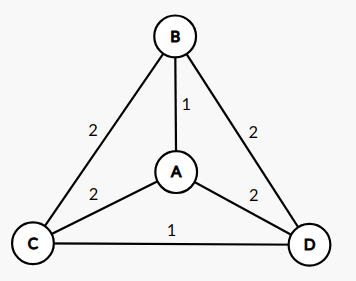
\includegraphics[width=0.3\textwidth]{graph.png}
	\caption{Exemplo de grafo}
	\label{graph}
\end{wrapfigure}

Por exemplo, para a figura \ref{graph}, um passeio fechado de custo ótimo seria: \[ \{A, B, D, C, A, D, C, B, A\} \], sendo este um caminho fechado de custo 12.
Neste exemplo foi necessário que as arestas $AB$ (ou $BA$) e $DC$ (ou $CD$) fossem percorridas duas vezes no passeio, porém nem sempre é necessária esta repetição.

No caso em que o grafo tratado é euleriano, a resposta para o problema do carteiro chinês é justamente o circuito euleriano do grafo.
Nos outros casos, sendo o grafo conexo, o procedimento que seguiremos será similar a realizar a cópia de algumas arestas do grafo de modo a torná-lo euleriano, ou seja, adicionar duplicatas de arestas até que todos os vértices possuam grau par.

Discutiremos nas seções a seguir a solução para o problema em questão com base nas especificidades do grafo do problema. 
Desconsideraremos nas análises a seguir grafos que possuam vértices isolados, isto é, vértices que não possuam arestas, já que tais vértices não afetam a solução do problema.

\subsection{Grafos não direcionados}

Analisaremos o caso em que o problema é modelado a partir de um grafo $G(V, E)$ simples, conexo e com arestas não direcionadas.

Um circuito Euleriano é um circuito que percorre todas arestas de $G$ exatamente uma vez. 
Já uma solução qualquer que resolva o problema do carteiro chinês deverá percorrer cada aresta de $G$ pelo menos uma vez, sendo assim uma trilha fechada.
Seja $1 + x_e$ o número de vezes que uma aresta $e \in E$ é percorrida em uma soluação $T$ do problema do carteiro chinês (PCC).

Se $G$ é euleriano, então a solução para o PCC é o próprio circuito euleriano do grafo.

Do contrário, definimos $G'$ como o grafo formado por $G$ adicionado de $x_e$ cópias de cada aresta $e \in E$. 
Isto é, cada aresta $e$ de $G$ aparecerá em $G'$ $1 + x_e$ vezes.
Deste modo, o grafo $G'$ será euleriano, e portanto a trilha euleriana de $G'$ corresponderá à solução do PCC para o grafo $G$.

Sendo assim, podemos separar a solução do PCC em duas partes: Encontrar o valor ótimo de $x_e$ para o problema descrito e, em seguida, encontrar um circuito euleriano no grafo $G'$ construído.

Resolveremos a primeira parte do problema com um algoritmo de emparelhamento.

%Seja $E(v)$ o conjunto de arestas ligadas ao vértice $v \in V$, e seja $c_e$ o custo de se percorrer uma aresta $e \in E$, que deverá ser não-negativo.

%Encontrar uma solução ótima para o PCC é equivalente a encontrar os valores inteiros e não negativos $x_e$ tal que $\sum_{e\in E(u)}(1 + x_e) \equiv 0 \mod 2$ para todo $u \in V$, minimizando o valor de $\sum_e c_ex_e$.

\begin{lemma} 
    \label{lemma-pcc}
    Para todo grafo simples e conexo, existirá uma solução ótima do PCC em que cada aresta é copiada no máximo 1 vez, ou seja que $x_e$ valerá apenas 0 ou 1. 
\end{lemma}

\begin{proof}
    Seja $T$ uma solução ótima do PCC para um grafo $G$ e $x$ um vetor indicando a quantidade de cópias necessárias de cada aresta de $G$ para a solução $T$. 
    Sabemos que $x$ deverá possuir valores inteiros não negativos, além disso, sabemos que o grafo $G'$, induzido por $x$, deverá ser euleriano e que o valor de $\sum_e c_ex_e$ será mínimo.

    Seja $x^*$ um vetor definido do seguinte modo:

    \[  x^*_e = x_e \bmod 2    \]

    Como o grafo $G'$ induzido por $x$ era euleriano, o grafo $G^*$ induzido por $x^*$ também deverá ser euleriano, pois a paridade dos vértices em ambos grafos é a mesma, e também pois tanto $G'$ quanto $G^*$ possuem $G$, que é conexo, como um subgrafo, e portanto também são conexos.
    
    Pela definição, $G^*$ usa um número menor ou igual de arestas duplicadas que $G'$, fazendo com que o seguinte se mantenha: $\sum_e c_ex^*_e \leq \sum_e c_ex_e$.

    No entanto, como $x$ foi derivado da solução ótima $T$, sabemos que $\sum_e c_ex_e$ deverá ser mínimo, e portanto, $\sum_e c_ex^*_e = \sum_e c_ex_e$. 

    Sendo assim, os valores de $x^*$ serão apenas 0 ou 1, por definição, e $T^*$ consistirá em uma solução ótima, assim como $T$, provando o lema.

\end{proof}

\begin{lemma}
    Para todo grafo $G$ simples e conexo, haverá uma solução ótima do PCC cujo conjunto de arestas duplicadas consistirá na união de caminhos aresta-disjuntos entre vértices de grau ímpar.
\end{lemma}

\begin{proof}

    Inicialmente trataremos o caso em que $G$ não possui nenhum vértice de grau ímpar:
    Se todos vértices de $G$ tem grau par, então o mesmo deve possuir um circuito euleriano. 
    Por isso, o vetor $x' = \{0, 0, \dots, 0\}$ induz uma solução válida para o PCC, e possui custo zero, sendo assim esta uma solução ótima.
    Como o conjunto de arestas duplicadas nesta solução é vazio, vale o lema para este grafo.

    Provado este caso, seguiremos a demonstração assumindo que $G$ possui ao menos um vértice de grau ímpar.

    Seja $T$ uma solução ótima do PCC para um grafo $G(V, E)$  em que cada aresta é copiada no máximo 1 vez, ou seja que $x_e$ valerá 0 ou 1. 
    A existência de tal solução é garantida pelo lema \ref{lemma-pcc}.
    Realizaremos uma prova por indução no número de arestas duplicadas de $G$, ou seja, em $\sum_e x_e$, para toda aresta $e \in E$. 

    O caso base dessa indução é quando $\sum_e x_e = 0$. 
    Neste caso, o conjunto de arestas duplicadas será vazio, valendo então a propriedade do lema.

    A hipótese de indução será que a propriedade do lema vale para uma soma $\sum_e x_e < k$, com $k > 0$.

    Analisaremos agora a situação em que $\sum_e x_e = k$, com $k > 0$.

    Seja $v$ um vértice de $G$ de grau ímpar,  $C$ um caminho de tamanho maximal que começa no vértice $v$ e percorre apenas arestas duplicadas e seja $G'$ o grafo, possivelmente desconexo, $G$ decrescido das arestas pertencentes a $C$.


    Todos os vértices em $G$ e $G'$ terão a mesma paridade de grau, exceto pelos vértices extremos de $C$. 
    Como estes eram vértices de grau ímpar em $G$ e apenas uma aresta foi retirada dos mesmos, ambos terão grau par em $G'$.

    Sendo assim, podemos definir um vetor $x'$ que induz uma solução ótima para $G'$ do seguinte modo:

    \[ 
        x'_e = 
        \begin{cases} 
            0 & e \in C \\
            x_e & e \notin C 
        \end{cases}
    \]


    Vale também o seguinte:

    \begin{align*}
        \sum_e x'_e &= \sum_e x_e - |\mathcal{C}| \\ 
        \sum_e x'_e &< \sum_e x_e \\
        \sum_e x'_e &< k
    \end{align*}

    Sendo assim, vale a hipótese de indução para o grafo $G'$, ou seja, existe um conjunto $\mathcal{C}$ de caminhos aresta-disjuntos entre vértices de grau ímpar composto por arestas duplicadas (ou seja, para as quais $x'_e = 1$).

    Como o grafo $G'$ não possui as arestas do caminho $C$, temos que todo caminho de $\mathcal{C}$ deverá ser aresta-disjunto com $C$.
    Deste modo, o conjunto de caminhos aresta-disjuntos entre vértices de grau ímpar $\mathcal{C} \cup C$, que induz o grafo $T$, consistirá de uma solução ótima para o PCC em $G$.
    Provando assim o passo da indução.

    Finalizando então a prova por indução do lema.

    \begin{figure}
        \centering
        \begin{tikzpicture}[auto,node distance=3cm, every loop/.style={},thick,main node/.style={circle,draw,font=\sffamily\Large}]
            \node[main node] (5) {5};
            \node[main node] (1) [below left of=5]{1};
            \node[main node] (2) [below of=1] {2};
            \node[main node] (4) [below right of=5] {4};
            \node[main node] (3) [below of=4] {3};

          \path[every node/.style={font=\sffamily\small}]
            (5) edge node [above] {0} (1)
            (5) edge node [above] {0} (4)
            (1) edge node [above] {0} (4)
            (2) edge node [right] {1} (1)
            (3) edge node [above] {1} (2)
            (4) edge node [left] {1} (3)
            ;
        \end{tikzpicture}
        \caption{Possível estrutura em grafo com vértices de grau ímpar}
        \label{pcc-case1}
    \end{figure}
    \begin{figure}
        \centering
        \begin{tikzpicture}[auto,node distance=3cm, every loop/.style={},thick,main node/.style={circle,draw,font=\sffamily\Large}]
            \node[main node] (1) {1};
            \node[main node] (2) [below of=1] {2};
            \node[main node] (4) [right of=1] {4};
            \node[main node] (3) [below of=4] {3};

          \path[every node/.style={font=\sffamily\small}]
            (1) edge node [above] {1} (4)
            (2) edge node [right] {1} (1)
            (3) edge node [above] {1} (2)
            (4) edge node [left] {1} (3)
            ;
        \end{tikzpicture}
        \caption{Caso em que o grafo tratado não possui vértices de grau ímpar}
        \label{pcc-case2}
    \end{figure}

\end{proof}

\begin{lemma}
    \label{lema-final}
    Para todo grafo $G$ simples e conexo, haverá uma solução ótima do PCC cujo conjunto de arestas duplicadas consistirá na união de caminhos de custo mínimo entre vértices de grau ímpar.
\end{lemma}

\begin{proof}
    Seja $S$ o conjunto de arestas duplicadas em uma solução ótima do PCC para o grafo $G$, que consiste de uma união de caminhos aresta-disjuntos entre vértices de grau ímpar.

    Imagine que um caminho $C$ pertencente a $S$, que liga os vértices quaisquer $u$ e $v$, não é o caminho mínimo entre os vértices que liga. 
    Isto é, existe um caminho $C'$ de custo menor que $C$ que liga $u$ e $v$.

    Neste caso, poderiamos retirar de $S$ as arestas do caminho $C$ e adicionar ao conjunto as arestas de $C'$. Deste modo, o conjunto $S$ possuiria um custo menor que o original, nos permitindo derivar de $S$ uma solução para o PCC de custo menor que a solução original.

    Porém, fazia parte da hipótese que a solução original era ótima, nos levando assim a uma contradição.

    Provamos assim o lema, garantindo a existência de uma solução para o PCC que consiste de uma união de caminhos mínimos entre vértices de grau ímpar.

\end{proof}

Um algoritmo que soluciona o problema se baseia em criar um novo grafo $G'(V', E')$. 
$V'$ é definido como o subconjunto de vértices de $V$ que possuem um grau ímpar em $G$, já $E'$ é definido como o conjunto de arestas entre todo par de vértices de $V'$, sendo que uma aresta entre dois vértices $u$ e $v$ quaisquer terá o custo igual ao custo de um caminho de menor custo entre os vértices $u$ e $v$ no grafo original $G$.


Pelo lema \ref{lema-final}, uma solução ótima do PCC em $G$ possui um conjunto de arestas duplicadas que pode ser representado como uma união de caminhos de custo mínimo entre vértices de grau ímpar. 
Como $V'$ é o conjunto dos vértices de grau ímpar em $G$ e cada aresta de $E'$ representa um caminho de custo mínimo entre dois vértices de $V'$, podemos reduzir o problema original à um problema de emparelhamento perfeito de custo mínimo no grafo $G'$.

Dado um emparelhamento perfeito $M$ em $G'$ de custo mínimo, é possível derivar uma solução ótima do PCC. Esta solução será dada por um circuito euleriano no grafo $G^*$ que construímos abaixo:

Considere $G^* = (V, E(G))$. Agora, para cada aresta $e = uv \in M$ (emparelhamento de $G'$), tome $C$ um caminho de custo mínimo de $u$ a $v$ em $G$ e faça $G^* \leftarrow G^* \cup C$, ou seja, duplique as arestas de $C$ em $G^*$.

A duplicação das arestas de um caminho modifica apenas a paridade dos vértices extremos.
Como, no procedimento acima, estamos duplicando as arestas de todos caminhos derivados do emparelhamento perfeito $M$, isso implica que moficamos a paridade de todos os vértices de $G^*$, ou seja, modificamos a paridade dos vértices de grau ímpar de $G$.

Sendo assim, o grafo $G^*$ resultante é euleriano, e a solução para o PCC do grafo $G$ é o circuito euleriano de $G^*$.



    % TODO: Expandir nesses assuntos:
        % Complexidade de um algoritmo
		%\item Essa solução não se aproveita do grafo ser esparso, há outra formulação do Edmonds e Johnson que leva isso em consideração.
		%\item Um problema similar é o de cobrir todas arestas com ciclos simples, de modo que o comprimento total dos ciclos é minimizado. Para grafos planares esses problemas são equivalentes.

    \subsection{Grafos direcionados}

    Analisaremos agora o problema do carteiro chinês aplicado a digrafos.

    \begin{lemma}
        Um digrafo $G$ possui solução para o problema do carteiro chinês se, e somente se, é fortemente conexo.
    \end{lemma}

    \begin{proof}


        ($\Rightarrow$) Começamos provando que para que um digrafo $G$ possua solução para o problema do carteiro chinês é necessário que o mesmo seja fortemente conexo.

        Vamos assumir, por absurdo, que $G$ possui uma solução para o PCC mas não é fortemente conexo.

        Como $G$ possui uma solução para o PCC, então existe um passeio fechado $T$ que passa por todos arcos de $G$.

         Além disso, como $T$ é um passeio fechado, para cada par de vértices $u, v$ de $G$, sabemos que $T$ passa por $u$ e $v$.
         Assim, $T = \{ v_0, v_1, \dots, v_i = u, \dots, v_j = v, \dots \}$.

        A partir de um passeio entre dois vértices sempre é possível derivar um caminho entre os mesmos seguindo o seguinte método:

        \begin{tcolorbox}
            \textbf{Método para derivar um caminho de um passeio qualquer}
            
            Seja $P$ um passeio que liga dois vértices quaisquer, mostraremos como construir um caminho ligando esses mesmos vértices a partir de $P$.

            Como $P$ é um passeio, possivelmente ele percorre um mesmo vértice mais que uma vez. Do contrário, já podemos considerar $P$ um caminho, finalizando o método. 

            Enquanto houver um vértice $v$ percorrido mais que uma vez por $P$ executa-se o seguinte passo:
    

            Retiramos de $P$ todos os vértices entre a primeira e a última aparição do vértice $v$, mantendo apenas tal vértice: 


            Portanto um passeio $P$ qualquer com repetição do vértice $v$, como o seguinte:
            \[
                P = \{ u_1, \dots u_i, v, \dots, v, u_j, \dots u_n\}
            \]

            Passa a ser:


            \[
                P = \{ u_1, \dots u_i, v, u_j, \dots u_n\}
            \]

            Repete-se tal passo até que $P$ não percorra um mesmo vértice duas vezes, se tornando assim, por definição, um caminho.

        \end{tcolorbox}
         
        Sendo assim, afirmamos que todo par de vértices presentes em $T$ possui um caminho entre si.

        Já que não estamos considerando neste trabalho digrafos que possuem vértices isolados, cada vértice de $G$ deve ser incidente ao menos a um arco. Além disso, como todos arcos são percorridos em $T$, já que ele é uma solução do PCC, todos os vértices deverão estar presentes no passeio fechado $T$.
        Por consequência para todo par de vértices de $G$ existe um caminho entre eles o que define $G$ como um grafo fortemente conexo, contradizendo a hipótese inicial.

        Provando assim que um digrafo que possua solução para o PCC é necessariamente fortemente conexo. \\

        ($\Leftarrow$)  Provaremos agora que todo grafo fortemente conexo $G$ possui uma solução para o PCC.

        Seja $v$ um vértice qualquer de $G$. Podemos construir uma solução $P$ para o problema do carteiro chinês do seguinte modo:


        Para qualquer arco $uw$ de $G$ definimos um circuito $C_{uw}$ que passa por $uw$ e pelo vértice $v$ como a concatenação do caminho de $v$ a $u$, do arco $uw$ e do caminho de $w$ a $v$.
        
        A existência de um caminho entre quaisquer dois vértices é garantida, já que $G$ é fortemente conexo, garantindo assim a existência de $C_{uw}$.
        
        Para construir a solução $P$, finalmente, basta realizar a concatenação dos circuitos $C_{e}$ para todo arco $e$ presente em $G$.

        Deste modo garantimos que toda aresta de $G$ é percorrida, provando assim a volta do lema: todo digrafo fortemente conexo possui uma solução para o problema do carteiro chinês.

    \end{proof}

    Em linhas gerais, o algoritmo que soluciona o problema do carteiro chinês para digrafos envolve multiplicar arestas do grafo original até que o mesmo se torne euleriano. O circuito euleriano desse digrafo modificado será a solução do problema do carteiro chinês para o digrafo original, do modo similar à solução para o PCC em grafos não direcionados.
    
    Uma grande diferença na solução do problema do carteiro chinês é que, para digrafos, não vale o lema \ref{lemma-pcc}, que garante a existência de uma solução para todo PCC em que cada aresta do grafo é percorrida no máximo duas vezes.
    Um contra-exemplo disso é o caso ilustrado na figura \ref{counter-lemma}. 

    \begin{figure}[h]
        \centering
        \begin{tikzpicture}[node distance=3cm, every loop/.style={},thick,main node/.style={circle,draw,font=\sffamily\Large}]
            \node[main node] (1) {1};
            \node[main node] (2) [right of=1] {2};
            \draw[edge] (1) to[bend left=50] (2);
            \draw[edge] (1) to[bend right=50] (2);
            \draw[edge] (1) to[] (2);
            \draw[edge] (2) to[bend left=100] (1);
        \end{tikzpicture}
        \caption{Contra exemplo do lema \ref{lemma-pcc} para os digrafos}
        \label{counter-lemma}
    \end{figure}

    Para que um passeio fechado percorra os três arcos de $1$ a $2$ da figura \ref{counter-lemma}, é necessário que esse mesmo passeio percorra três vezes o arco de $2$ a $1$.

    O lema \ref{lemma-pcc} é utilizado para justificar a utilização de um algoritmo de emparelhamento perfeito para definir quais arestas duplicar na solução do PCC.
    Como tal lema não vale para digrafos, a escolha dessas arestas deverá ser feita de um modo diferente, utilizando um algoritmo de fluxo máximo de custo mínimo, como veremos a seguir, no detalhamento do algoritmo que soluciona o PCC.

    \begin{tcolorbox}
	\textbf{Solução:}

    A solução do PCC para um digrafo $G$ fortemente conexo pode ser dividida em 4 passos:

    \begin{enumerate}
        % TODO: ARRUAMR TODAS AS DEFINICOES DE F S
        \item[\textbf{1º}] Definimos como $F$ o conjunto dos vértices que possuam grau de saída maior que o grau de entrada e $S$ o conjunto dos vértices que possuam grau de entrada maior que o grau de saída.

    Computamos então o custo do menor caminho entre todos os pares de vértices $u, v$ onde $u \in F$ e $v \in S$.


        \item[\textbf{2º}] Modelamos então um problema de transporte: 
        Os vértices de $F$ serão vértices de oferta, cada vértice $u \in F$ terá que escoar $\delta^-(u) - \delta^+(u)$ unidades de fluxo, já os vértices de $S$ serão vértices de demanda, cada vértice $v \in S$ terá que receber $\delta^+(v) - \delta^-(v)$ unidades de fluxo.

        Todo par de vértices $u, v$ com $u \in F$ e $v \in S$ será ligado por um arco de capacidade infinita e custo igual ao custo de um menor caminho de $u$ a $v$, calculado no primeiro passo.

        Deve-se então resolver tal problema de transporte minimizando o custo total.

        \item[\textbf{3º}] A partir de uma solução ótima encontrada para o problema de transporte devemos derivar um digrafo euleriano baseado em $G$.

            Cada arco $uv$ criado na modelagem do problema de transporte representa um caminho de mesmo custo no digrafo $G$ entre os vértices $u$ e $v$. Se um arco da modelagem é escolhido para a solução que estamos analisando, então todos arcos do caminho que tal arco condensado representa devem ser duplicados no digrafo $G$.

            Após a duplicação dos arcos de um caminho entre dois vértices $u$ e $v$ a diferença absoluta dos graus de entrada e saída de $u$ e $v$ diminuirão em uma unidade, essa mesma diferença de graus se manterá constante para vértices internos ao caminho. 

            Ao final das duplicações necessárias, todos vértices de $G$ possuirão um mesmo valor de grau de entrada e saída, sendo assim euleriano segundo o teorema \ref{euler-digraph}.

        \item[\textbf{4º}] Encontrar o circuito euleriano do novo grafo $G$, que será também a solução do problema do carteiro chinês para o grafo original $G$.

    \end{enumerate}

    \end{tcolorbox}
    Aplicaremos agora o passo a passo apresentado acima em um exemplo. 

    \begin{figure}[H]
        \centering
        \begin{tikzpicture}[node distance=3cm, every loop/.style={},thick,main node/.style={circle,draw,font=\sffamily\Large}]

            \node[main node] (d) {d};
            \node[main node] at (-4, 1) (g) {g};
            \node[main node] at (-2, 3) (f) {f};
            \node[main node] at (2, 3) (c) {c};
            \node[main node] at (5, 0) (a) {a};
            \node[main node] at (-2, -3) (e) {e};
            \node[main node] at (2, -3) (b) {b};

            \path[->] (a) edge[bend right, below] node {4} (b);
            \path[->] (a) edge[below] node {9} (d);
            \path[->] (a) edge[below] node {4} (c);
            \path[->] (b) edge[below] node {5} (a);
            \path[->] (c) edge[bend right, above] node {6} (d);
            \path[->] (c) edge[above] node {8} (f);
            \path[->] (d) edge[below] node {3} (e);
            \path[->] (d) edge[bend right, below] node {6} (c);
            \path[->] (e) edge[below] node {6} (b);
            \path[->] (e) edge[below] node {5} (g);
            \path[->] (f) edge[below] node {4} (g);
            \path[->] (g) edge[above] node {6} (d);
        \end{tikzpicture}
        \caption{Digrafo retirado de exercício do site do MIT\cite{mit}}
        \label{konigsberg-graph}
    \end{figure}


    \begin{itemize}
        \item[\textbf{1º}] 
            Definimos então os conjuntos $F$ e $S$:

            \[
                F  = \{b, d, g\}
            \]
            \[
                S =  \{a, e\}
            \]

            Computamos também a distância mínima entre os pares de vértices dos dois conjuntos:

            \begin{center}
                \begin{tabular}{ |p{1cm}||p{1cm}|p{1cm}|  }
                    \hline
                     & a & e \\
                    \hline
					\hline
                    b & 4 & 17 \\
                    \hline
                    d & 14 & 3 \\
                    \hline
                    g & 20 & 9\\
                    \hline
                \end{tabular}
            \end{center}

        \item[\textbf{2º}]

            Modelamos então o problema de transporte, os vértices $b, d, g$ escoando uma unidade de fluxo cada e os vértices $a, b$ com demandas 2 e 1, respectivamente.

            \begin{figure}[H]
                \centering
                \begin{tikzpicture}[node distance=3cm, every loop/.style={},thick,main node/.style={circle,draw,font=\sffamily\Large}]

					\node[main node] (1) {b};
					\node (v1) at(-0.75, 0) {1};
					\node[main node] at (0, -2) (2) {d};
					\node (v2) at(-0.75, -2) {1};
					\node[main node] at (0, -4) (3) {g};
					\node (v3) at(-0.75, -4) {1};

					\node[main node] at(3, -1) (4) {a};
					\node (v4) at(3.75, -1) {2};
					\node[main node] at(3, -3) (5) {e};
					\node (v5) at(3.75, -3) {1};

                    \path[->] (1) edge node[pos=0.25,above] {4} (4);
                    \path[->] (1) edge node[pos=0.25,above] {17} (5);
                    \path[->] (2) edge node[pos=0.20,above] {14} (4);
                    \path[->] (2) edge node[pos=0.25,above left] {3} (5);
                    \path[->] (3) edge node[pos=0.20,above] {20} (4);
                    \path[->] (3) edge node[pos=0.25,above] {9} (5);
                \end{tikzpicture}
            \end{figure}

            Os arcos definidos entre os vértices de $F$ e $S$ possuem capacidade infinita e custo igual à distância mínima dos mesmos vértices em $G$, como já calculado no primeiro passo.

            Uma solução ótima para o problema apresentado consiste em utilizar os arcos de custo $4, 14$ e $9$, escoando assim toda a demanda dos vértices $b, d$ e $g$.

            \begin{figure}[H]
                \centering
                \begin{tikzpicture}[node distance=3cm, every loop/.style={},thick,main node/.style={circle,draw,font=\sffamily\Large}]

					\node[main node] (1) {b};
					\node (v1) at(-0.75, 0) {1};
					\node[main node] at (0, -2) (2) {d};
					\node (v2) at(-0.75, -2) {1};
					\node[main node] at (0, -4) (3) {g};
					\node (v3) at(-0.75, -4) {1};

					\node[main node] at(3, -1) (4) {a};
					\node (v4) at(3.75, -1) {2};
					\node[main node] at(3, -3) (5) {e};
					\node (v5) at(3.75, -3) {1};

                    \path[->] (1) edge[red] node[pos=0.25,above] {4} (4);
                    \path[->] (1) edge node[pos=0.25,above] {17} (5);
                    \path[->] (2) edge[red] node[pos=0.20,above] {14} (4);
                    \path[->] (2) edge node[pos=0.25,above left] {3} (5);
                    \path[->] (3) edge node[pos=0.20,above] {20} (4);
                    \path[->] (3) edge[red] node[pos=0.25,above] {9} (5);
                \end{tikzpicture}
            \end{figure}

        \item[\textbf{3º}] Agora devemos realizar a duplicação dos caminhos representados pelas arestas $ba, da$ e $ge$.

            Representamos o estado inicial do digrafo $G$, sem os pesos nos arcos:

            \begin{figure}[H]
                \centering
                \begin{tikzpicture}[node distance=3cm, every loop/.style={},thick,main node/.style={circle,draw,font=\sffamily\Large}]

					\node[main node] (d) {d};
					\node[main node] at (-4, 1) (g) {g};
					\node[main node] at (-2, 3) (f) {f};
					\node[main node] at (2, 3) (c) {c};
					\node[main node] at (5, 0) (a) {a};
					\node[main node] at (-2, -3) (e) {e};
					\node[main node] at (2, -3) (b) {b};

					\path[->] (a) edge[bend right, below] node {} (b);
					\path[->] (a) edge[below] node {} (d);
					\path[->] (a) edge[below] node {} (c);
					\path[->] (b) edge[below] node {} (a);
					\path[->] (c) edge[bend right, above] node {} (d);
					\path[->] (c) edge[above] node {} (f);
					\path[->] (d) edge[below] node {} (e);
					\path[->] (d) edge[bend right, below] node {} (c);
					\path[->] (e) edge[below] node {} (b);
					\path[->] (e) edge[below] node {} (g);
					\path[->] (f) edge[below] node {} (g);
                    \path[->] (g) edge[above] node {} (d);
                \end{tikzpicture}
            \end{figure}

            Faremos tal duplicação passo a passo, começando a duplicar os arcos do caminho mínimo de $b$ a $a$. Representamos as arestas adicionadas em vermelho.


            \begin{figure}[H]
                \centering
                \begin{tikzpicture}[scale=0.7, every node/.style={scale=0.7},node distance=3cm, every loop/.style={},thick,main node/.style={circle,draw,font=\sffamily\Large}]

					\node[main node] (d) {d};
					\node[main node] at (-4, 1) (g) {g};
					\node[main node] at (-2, 3) (f) {f};
					\node[main node] at (2, 3) (c) {c};
					\node[main node] at (5, 0) (a) {a};
					\node[main node] at (-2, -3) (e) {e};
					\node[main node] at (2, -3) (b) {b};

					\path[->] (a) edge[bend right, below] node {} (b);
					\path[->] (a) edge[below] node {} (d);
					\path[->] (a) edge[below] node {} (c);
					\path[->] (b) edge[below] node {} (a);
					\path[->] (b) edge[red, bend right, below] node {} (a);
					\path[->] (c) edge[bend right, above] node {} (d);
					\path[->] (c) edge[above] node {} (f);
					\path[->] (d) edge[below] node {} (e);
					\path[->] (d) edge[bend right, below] node {} (c);
					\path[->] (e) edge[below] node {} (b);
					\path[->] (e) edge[below] node {} (g);
					\path[->] (f) edge[below] node {} (g);
                    \path[->] (g) edge[above] node {} (d);
                \end{tikzpicture}
            \end{figure}

    Agora duplicaremos os arcos do caminho mínimo de $d$ a $a$:

    \begin{figure}[H]
        \centering
        \begin{tikzpicture}[scale=0.7, every node/.style={scale=0.7},node distance=3cm, every loop/.style={},thick,main node/.style={circle,draw,font=\sffamily\Large}]

            \node[main node] (d) {d};
            \node[main node] at (-4, 1) (g) {g};
            \node[main node] at (-2, 3) (f) {f};
            \node[main node] at (2, 3) (c) {c};
            \node[main node] at (5, 0) (a) {a};
            \node[main node] at (-2, -3) (e) {e};
            \node[main node] at (2, -3) (b) {b};

            \path[->] (a) edge[bend right, below] node {} (b);
            \path[->] (a) edge[below] node {} (d);
            \path[->] (a) edge[below] node {} (c);
            \path[->] (b) edge[below] node {} (a);
            \path[->] (b) edge[bend right, below] node {} (a);
            \path[->] (b) edge[red, bend right=60, below] node {} (a);
            \path[->] (c) edge[bend right, above] node {} (d);
            \path[->] (c) edge[above] node {} (f);
            \path[->] (d) edge[below] node {} (e);
            \path[->] (d) edge[red, bend right, below] node {} (e);
            \path[->] (d) edge[bend right, below] node {} (c);
            \path[->] (e) edge[below] node {} (b);
            \path[->] (e) edge[red, bend right, below] node {} (b);
            \path[->] (e) edge[below] node {} (g);
            \path[->] (f) edge[below] node {} (g);
            \path[->] (g) edge[above] node {} (d);
        \end{tikzpicture}
    \end{figure}

    Finalmente, duplicamos os arcos do caminho mínimo de $g$ a $e$:


    \begin{figure}[H]
        \centering
        \begin{tikzpicture}[scale=0.7, every node/.style={scale=0.7},node distance=3cm, every loop/.style={},thick,main node/.style={circle,draw,font=\sffamily\Large}]

            \node[main node] (d) {d};
            \node[main node] at (-4, 1) (g) {g};
            \node[main node] at (-2, 3) (f) {f};
            \node[main node] at (2, 3) (c) {c};
            \node[main node] at (5, 0) (a) {a};
            \node[main node] at (-2, -3) (e) {e};
            \node[main node] at (2, -3) (b) {b};

            \path[->] (a) edge[bend right, below] node {} (b);
            \path[->] (a) edge[below] node {} (d);
            \path[->] (a) edge[below] node {} (c);
            \path[->] (b) edge[below] node {} (a);
            \path[->] (b) edge[bend right, below] node {} (a);
            \path[->] (b) edge[bend right=60, below] node {} (a);
            \path[->] (c) edge[bend right, above] node {} (d);
            \path[->] (c) edge[above] node {} (f);
            \path[->] (d) edge[below] node {} (e);
            \path[->] (d) edge[bend right, below] node {} (e);
            \path[->] (d) edge[red, bend left, below] node {} (e);
            \path[->] (d) edge[bend right, below] node {} (c);
            \path[->] (e) edge[below] node {} (b);
            \path[->] (e) edge[bend right, below] node {} (b);
            \path[->] (e) edge[below] node {} (g);
            \path[->] (f) edge[below] node {} (g);
            \path[->] (g) edge[above] node {} (d);
            \path[->] (g) edge[red, bend left, above] node {} (d);
        \end{tikzpicture}
    \end{figure}

    As sucessivas duplicações de caminho realizadas em $G$ fazem com que todos os vértices possuam grau de saída e entrada iguais. Pelo teorema \ref{euler-digraph} temos que o novo grafo é euleriano. No quarto passo derivaremos um circuito euleriano para o digrafo construído.


\item[\textbf{4º}]  Um possível circuito eulerian $\mathcal{C}$ que se inicia no vértice $a$ é o seguinte:

    \[ 
        \mathcal{C} = \{ a, c, f, g, d, c, d, e, g, d, e, b, a, d, e, b, a, b, a \}
    \]

    Representamos tal circuito no grafo abaixo, indicando em cada arco a ordem em que o mesmo é percorrido:

    \begin{figure}[H]
        \centering
        \begin{tikzpicture}[node distance=3cm, every loop/.style={},thick,main node/.style={circle,draw,font=\sffamily\Large}]

            \node[main node] (d) {d};
            \node[main node] at (-4, 1) (g) {g};
            \node[main node] at (-2, 3) (f) {f};
            \node[main node] at (2, 3) (c) {c};
            \node[main node] at (5, 0) (a) {a};
            \node at(6, 1) (st) {início};
            \node[main node] at (-2, -3) (e) {e};
            \node[main node] at (2, -3) (b) {b};

            \path[->] (st) edge[] node {} (a);

            \path[->] (a) edge[bend right, below] node {17} (b);
            \path[->] (a) edge[above] node {13} (d);
            \path[->] (a) edge[below] node {1} (c);
            \path[->] (b) edge[below] node {18} (a);
            \path[->] (b) edge[red, bend right, below] node {16} (a);
            \path[->] (b) edge[red, bend right=60, below] node {12} (a);
            \path[->] (c) edge[bend right, above] node {6} (d);
            \path[->] (c) edge[above] node {2} (f);
            \path[->] (d) edge[below] node {10} (e);
            \path[->] (d) edge[red, bend right, above] node {7} (e);
            \path[->] (d) edge[red, bend left, below] node {14} (e);
            \path[->] (d) edge[bend right, below] node {5} (c);
            \path[->] (e) edge[below] node {15} (b);
            \path[->] (e) edge[red, bend right, below] node {11} (b);
            \path[->] (e) edge[below] node {8} (g);
            \path[->] (f) edge[below] node {3} (g);
            \path[->] (g) edge[above] node {9} (d);
            \path[->] (g) edge[red, bend left, above] node {4} (d);
        \end{tikzpicture}
        \caption{Representa-se em preto os arcos presentes no grafo $G$ original, e em vermelho os arcos resultantes das duplicações realizadas no terceiro passo da solução.}
    \end{figure}

    O circuito $\mathcal{C}$ percorrido no grafo original $G$ representa o passeio fechado que soluciona o Problema do Carteiro Chinês, já que percorre todo arco de $G$ ao menos uma vez.

    Analisando o peso dos arcos de $G$ concluimos que a solução $\mathcal{C}$ tem custo $66+27 = 93$, $66$ é o custo de se percorrer todas os arcos de $G$, representados em preto, uma única vez, e $27$ é o custo de se percorrer alguns arcos mais que uma vez.

    \end{itemize}

    \subsection{Grafos mistos}

    Já analisamos o Problema do Carteiro Chinês aplicado a grafos e digrafos, agora discutiremos o mesmo problema aplicado a grafos mistos, ou seja, grafos que tenham tanto arestas quanto arcos.

    Ao contrário do que uma análise breve pode sugerir, não é possível reduzir o PCC para grafos mistos ao caso de grafos direcionados simplesmente transformando as arestas não direcionadas em dois arcos de sentidos opostos.

    Um contra-exemplo para este pensamento é o seguinte:

    \begin{center}
        \begin{tikzpicture}[node distance=2cm, every loop/.style={},thick,main node/.style={circle,draw,font=\sffamily\Large}]
            \node[main node] (1) {1};
            \node[main node] (2) [below of=1] {2};
            \path[->] (2) edge[bend right] node {} (1);
            \path[-] (2) edge[bend left] node {} (1);
        \end{tikzpicture}
        \hspace{3cm}% NO SPACE!
        \begin{tikzpicture}[node distance=2cm, every loop/.style={},thick,main node/.style={circle,draw,font=\sffamily\Large}]
            \node[main node] (1) {1};
            \node[main node] (2) [below of=1] {2};
            \path[->] (2) edge[bend right] node {} (1);
            \path[->] (2) edge[bend left] node {} (1);
            \path[->] (1) edge[bend right=60] node {} (2);
        \end{tikzpicture}
    \end{center}

    Na esquerda temos um grafo não direcionado qualquer, e na direita temos o mesmo grafo com sua aresta substituida por dois arcos em sentidos opostos. 

    Apesar da similaridade dos grafos, suas soluções para o problema do carteiro chinês diferem.
    \sloppy Uma solução do problema para o primeiro grafo é $\{1, 2, 1\}$, enquanto que uma solução possível para o segundo grafo é $\{1, 2, 1, 2, 1\}$, como representado visualmente a seguir.

    \begin{center}
        \begin{tikzpicture}[node distance=2cm, every loop/.style={},thick,main node/.style={circle,draw,font=\sffamily\Large}]
            \node[main node] (1) {1};
            \node[main node] (2) [below of=1] {2};
            \path[->] (2) edge[left, bend right] node {2} (1);
            \path[-] (2) edge[left, bend left] node {1} (1);
        \end{tikzpicture}
        \hspace{3cm}% NO SPACE!
        \begin{tikzpicture}[node distance=2cm, every loop/.style={},thick,main node/.style={circle,draw,font=\sffamily\Large}]
            \node[main node] (1) {1};
            \node[main node] (2) [below of=1] {2};
            \path[->] (2) edge[right, bend right] node {2} (1);
            \path[->] (2) edge[right, bend left] node {4} (1);
            \path[->] (1) edge[left, bend right=60] node {1, 3} (2);
        \end{tikzpicture}
    \end{center}

    Apesar de conseguirmos encontrar uma solução para o caso direcionado derivado, não há um modo trivial de transformar uma solução para tal caso em uma solução do caso não direcionado.

    Diferentemente dos grafos ou digrafos, o PCC aplicado a grafos mistos não possui solução polinomial, sendo um problema NP-hard. 



    % TODO: Adicionar a discussao de que nao da pra transformar esse em um caso direcionado

	NP-hard, mesmo se $G$ for planar e se todos $c_{ij}$ forem iguais.

    \section{Problemas resolvidos}

        Esta seção se dedica a discutir aplicações do Problema do Carteiro Chinês em problemas de competições de programação.

        \subsection{Sereja and the Arrangement of Numbers\cite{sereja}}

        \textbf{Definição do problema}

        No enunciado do problema define-se uma sequência $s$ como \textbf{bonita} quando existe um inteiro $i$ para cada par de valores distintos $u$, $v$ pertencentes a $s$, tal que $s_i = u, s_{i+1} = v$ ou $s_i = v, s_{i+1} = u$.

        Em outras palavras, se uma sequência é bonita todo par de valores distintos pertencentes à essa sequência aparecem na mesma lado a lado ao menos uma vez.

        Define-se também um sistema de recompensas:
        Para cada valor há uma recompensa positiva associada.
        A recompensa total de uma sequência é igual à soma das recompensas de seus valores distintos, ou seja, a recompensa não depende do número de vezes que cada valor aparece na sequência.

        O problema consiste então desenvolver um algoritmo que calcule a maior recompensa atingível para uma sequência bonita de tamanho $n$ que seja constituída apenas por valores definidos pela entrada. 

        A entrada do programa, portanto será dada pelos valores $n, m$ e por $m$ pares $q_i, w_i$, indicando que $q_i$ é um valor que pode ser utilizado e que possui recompensa $w_i$, garante-se que os valores de $q_i$ são distintos e que $w_i$ é positivo.

        Um exemplo de entrada para este problema é:

        \begin{align*}
            & 5 \text{ }4 & \text{Neste exemplo $n = 5$ e $m = 4$}\\
            & 1 \text{ }4 & \text{O primeiro valor é 1, e sua recompensa é 4}\\
            & 2 \text{ }3 & \text{Segue o valor 2, com recompensa 3}\\
            & 4 \text{ }2 & \text{Segue o valor 4, com recompensa 2}\\
            & 3 \text{ }10 &\text{Finalmente temos o valor 3, de recompensa 10}\\
        \end{align*}

        Para este exemplo, uma solução ótima é a sequência $1,2,3,1,1$, que é bonita e possui recompensa total igual a $17$. 
        Não existe uma sequência bonita que possua os quatro valores do exemplo.


        \textbf{Descrição da solução}

        Como todo valor possui uma recompensa positiva, a solução final deverá usar a maior quantidade de valores distintos que for possível.

        Começaremos discutindo um problema mais simples: Qual o tamanho da menor sequência bonita que utiliza $x$ valores distintos?

        Para resolver esse problema faremos uma modelagem do problema usando um grafo completo $K_x$, que possui $x$ vértices, onde cada vértice representa um valor distinto e cada aresta possui custo unitário.

        Todo passeio do grafo $K_x$ pode ser representado como uma sequência dos valores dos vértices do grafo, as sequências definidas como bonitas são aquelas que representam um passeio que percorre todas arestas do grafo $K_x$.

        Para facilitar a análise deste problema, assumiremos que pode existir em um passeio dois vértices de mesmo valor em sequência, mesmo sem haver um loop neste vértice, além disso, vamos assumir que os valores distintos são $1, 2, \dots, x$.

        Sendo assim, podemos interpretar uma sequência $s$ que possua apenas valores entre $1$ e $x$ como um passeio em $K_x$, os valores da sequência representam os vértices do grafo $K_x$, e dois valores adjacentes $u$ e $v$ representam que a aresta $uv$ está presente no passeio derivado de $s$. 
        
        Para que a sequência $s$ seja bonita, todo par de valores distintos $u, v$ deverá aparecer ao menos uma vez lado a lado, o que implica que o passeio derivado de $s$ deverá percorrer a aresta $uv$ ao menos uma vez.

        Concluimos então que um passeio derivado de uma sequência que seja bonita, deverá percorrer todas arestas do grafo $K_x$, sendo assim uma solução do problema do carteiro chinês para o mesmo.

        Voltamos assim à pergunta inicial, a menor sequência bonita que utiliza $x$ valores distintos, será aquela que representa uma solução ótima do problema do carteiro chinês para o grafo $K_x$, já que a solução que miniza o custo do PCC também minimizará o número de arestas percorridas, e portantom, o tamanho da sequência bonita. \\
 
        Vejamos agora alguns exemplos:

        \begin{figure}[h]
            \centering
            \begin{tikzpicture}[auto,node distance=3cm, every loop/.style={},thick,main node/.style={circle,draw,font=\sffamily\Large}]
                \node[main node] (1) {1};
                \node[main node] (2) [below left of=1] {2};
                \node[main node] (3) [below of=2] {3};
                \node[main node] (5) [below right of=1] {5};
                \node[main node] (4) [below of=5] {4};

                \path[every node/.style={font=\sffamily\small}]
                    (1) edge node [] {} (4)
                    (1) edge node [] {} (3)
                    (2) edge node [] {} (1)
                    (1) edge node [] {} (5)
                    (2) edge node [] {} (4)
                    (3) edge node [] {} (2)
                    (2) edge node [] {} (5)
                    (4) edge node [] {} (3)
                    (3) edge node [] {} (5)
                    (4) edge node [] {} (5)
                    ;
            \end{tikzpicture}
            \caption{Exemplo com $x=5$}
            \label{k5}
        \end{figure}

        Para $x=5$, o grafo induzido é o $K_5$, como representado na figura \ref{k5}.
        Como todos os vértices do $K_5$ possuem grau par, a solução ótima do Problema do Carteiro Chinês para este exemplo é também um circuito euleriano, como o seguinte:


        \[ P = \{1, 2, 3, 4, 5, 1, 3, 5, 2, 4, 1\} \]

        Como discutido anteriormente, $P$, além de solução do PCC é também uma sequência bonita que utiliza os $x$ valores definidos pelos vértices do grafo.
        
        Sendo assim, para utilizar $5$ valores distintos, é necessário ter uma sequência de tamanho no mínimo $11$, valor este que é igual a $1 + |E(K_5)| = 1 + 10 = 11$.

        Analisaremos agora outro exemplo, em que $x=4$, do qual se deriva o grafo $K_4$ representado na figura \ref{k4}.


        \begin{figure}[h]
            \centering
            \begin{tikzpicture}[auto,node distance=3cm, every loop/.style={},thick,main node/.style={circle,draw,font=\sffamily\Large}]
                \node[main node] (1) {1};
                \node[main node] (2) [below of=1] {2};
                \node[main node] (4) [right of=1] {4};
                \node[main node] (3) [below of=4] {3};

                \path[every node/.style={font=\sffamily\small}]
                    (1) edge node {} (4)
                    (2) edge node {} (1)
                    (3) edge node {} (2)
                    (4) edge node {} (3)
                    (1) edge node {} (3)
                    (2) edge node {} (4)
                    ;
            \end{tikzpicture}
            \caption{Exemplo com $x=4$}
            \label{k4}
        \end{figure}


        Neste exemplo, todos os vértices de $K_4$ possuem grau ímpar, por isso, a primeira parte da solução do problema do carteiro chinês se baseia em duplicar algumas arestas do grafo, tornando-o um grafo euleriano.

        Como estamos tratando de um grafo completo, com arestas de custo unitário, não é necessário criar uma condensação do grafo $K_x$, e achar um emparelhamento perfeito de custo mínimo.
        Basta apenas criar uma duplicação de aresta entre todo par de vértices de índices $i$ e $i+1$ para todo índice $i$ ímpar, como representado na figura \ref{k4+} para o exemplo em questão.

        \begin{figure}[h]
            \centering
            \begin{tikzpicture}[auto,node distance=3cm, every loop/.style={},thick,main node/.style={circle,draw,font=\sffamily\Large}]
                \node[main node] (1) {1};
                \node[main node] (2) [below of=1] {2};
                \node[main node] (4) [right of=1] {4};
                \node[main node] (3) [below of=4] {3};

                \path[every node/.style={font=\sffamily\small}]
                    (1) edge[] node {} (4)
                    (2) edge[bend right] node {} (1)
                    (4) edge[bend right] node {} (3)
                    (1) edge node {} (3)
                    (2) edge node {} (4)
                    (2) edge node {} (3)
                    (1) edge[bend right] node {} (2)
                    (3) edge[bend right] node {} (4)
                    ;
            \end{tikzpicture}
            \caption{$K_4$ com arestas duplicadas}
            \label{k4+}
        \end{figure}

        A partir do grafo euleriano criado, é possível encontrar o caminho euleriano $P$, que também é solução do PCC para o grafo $K_4$, e, finalmente, sequência bonita de tamanho mínimo que usa $4$ valores distintos.

        \[ P = \{1, 2, 3, 4, 1, 3, 4, 2, 1\} \]

        Sendo assim, o tamanho mínimo de uma sequência bonita que possui 4 valores distintos é $9$, valor este composto da seguinte forma: $1 + |E(K_4)| = 1 + 6 = 7$ somado ao número de arestas duplicadas $\frac{4}{2} = 2$.


        Podemos assim abstrair uma fórmula geral para o tamanho mínimo de uma sequência bonita $P$ que utilize $k$ valores distintos em sua composição:

        
        \[ |P|
             =  1 + \frac{k(k-1)}{2} + 
            \begin{cases} 
                0 & k \text{ ímpar} \\
                \frac{k}{2} & k \text{ par}
            \end{cases}
        \]

        Todo grafo completo com uma quantidade ímpar de vértices é euleriano, já que todos seus vértices possuem grau par, enquanto os grafos completos com quantidade par de vértices não são eulerianos. 
        Por isso a diferença na fórmula de $|P|$.

        A partir dessa fórmula fechada, é possível descobrir com uma busca binária, em complexidade $\mathcal{O}(\lg{n})$, qual o maior valor de $k$ tal que $|P| \leq n$.

        Encontrado tal valor $k$, o número máximo de valores distintos que a solução pode possuir para ser bonita, basta descobrir quais valores da entrada escolher para maximizar a recompensa.
        

        Se possuirmos na entrada uma quantidade de valores, $m$, tal que $m \leq k$, então a solução ótima será a soma das recompensas de todos valores, já que é possível encontrar uma sequência bonita que irá conter todos valores disponíveis.

        Do contrário, a solução consistirá em escolher os $k$ valores de maior recompensa disponíveis.
    Para encontrar tal valor, basta manter uma árvore de busca binária balanceada com as $k$ maiores recompensas dos valores disponíveis, o que custa tempo $\mathcal{O}(m\lg k) = \mathcal{O}(m\lg \sqrt{n})$.

    Uma solução para este problema foi adicionada a referência \cite{sereja-sol}. 

        \subsection{Jogging Trails\cite{jogging}}
        
        Neste problema devemos desenvolver um programa que calcula o custo de uma solução ótima para o problema do carteiro chinês em um grafo não direcionado de até 15 vértices com pesos nas arestas.

        Este problema é uma aplicação direta do problema descrito nesse trabalho. 
        Entretanto, em virtude do limite do número de vértices das instâncias, é possível resolver o problema de maneira mais simples.

        Um dos últimos passos do algoritmo que resolve o problema do carteiro chinês em grafos não direcionados descrito neste trabalho é realizar a condensação do grafo original usando os vértices de grau ímpar e posteriormente cosntruir o emparelhamento perfeito de custo mínimo usando o algoritmo de Edmonds.

        Uma alternativa viável para este problema é realizar a construção do emparelhamento perfeito usando, ao invés do algoritmo de Edmonds, um algoritmo de programação dinâmica:

         Para esta solução devemos memoizar o custo mínimo de emparelhamento perfeito para todo subconjunto de vértices do grafo condensado.

        Seja $K$ o grafo completo condensado, $S$ um subconjunto dos vértices de $K$, $dist$ uma função que retorna a distância entre dois vértices quaisquer de $K$ e $min\_cost_S$ o menor custo de emparelhamento perfeito do subconjunto $S$ de vértices, podemos definir a seguinte recorrência:

        \[
            min\_cost_S = 
            \begin{cases} 
                0 & S = \{ \} \\
                \min_{u, v \in S} min\_cost_{S - u - v} + dist(u, v) & \text{caso contrário}
            \end{cases}
        \]

        Para representar os subconjuntos de vértices pode-se utilizar uma bitmask.
        Como foi utilizado na solução\cite{jogging-sol} adicionada à referência.



	\section{Windy Postman Problem}

	NP-hard

	Se todo ciclo do grafo tem o mesmo custo em ambos sentidos, transforma a aresta entre $i$ e $j$ de custos $c_{ij}$ e $c_{ji}$ em uma aresta não direcionada com custo $\frac{c_{ij} + c_{ji}}{2}$. Essa transformação reduz o problema de a um CPP não direcionado, que tem solução polinomial, porém para isso é necessário checar se todo ciclo tem o mesmo custo nas duas direções.

	\section{Hierarchical Postman Problem}

	NP-hard 

	Seja $P = \{A_1, A_2, \dots, A_k\}$ uma partição do conjunto de arestas $A$. Determinar um caminho em $G$ de custo mínimo que sai de um vértice $s$ e atinge um vértice $t$, respeitando uma hierarquia das arestas. O caminho só poderá possuir uma aresta pertencente a $A_j$ se o caminho passar anteriormente por todas arestas pertencentes a $A_i$, se $i < j$.


	\section{Anotações}

	\begin{itemize}
		\item Todo mixed CPP pode ser transformado em um WPP.
	\end{itemize}

	\medskip

	\begin{thebibliography}{9}
	\bibitem{konigsberg} 
	Euler, Leonhard
	\textit{Solution problematis ad geometriam situs pertinentis}. 
	Comment. Acad. Sci. U. Petrop 8, 128–40, 1736.

	\bibitem{hierholzer}
	Hierholzer, Carl
	\textit{``Über die Möglichkeit, einen Linienzug ohne Wiederholung und ohne Unterbrechung zu umfahren''}, 
	Mathematische Annalen, 6 (1): 30–32, doi:10.1007/BF01442866, 1873.

    \bibitem{sereja}
    Problema retirado do Codeforces, problema C do Round \#215 (Div1)\\
    \href{https://codeforces.com/problemset/problem/367/C}{codeforces.com/problemset/problem/367/C}

    \bibitem{sereja-sol}
    Solução para o problema Sereja and the Arrangement of Numbers, desenvolvida em C++\\
    \href{https://github.com/gafeol/competitive-programming/blob/master/ojs/cf/367/C.cpp}{github.com/gafeol/competitive-programming/blob/master/ojs/cf/367/C.cpp}

    \bibitem{jogging}
    Problema retirado do UVa, problema 10296\\
    \href{https://onlinejudge.org/index.php?option=com_onlinejudge&Itemid=8&page=show_problem&problem=1237}{onlinejudge.org/index.php?option=com\_onlinejudge\&Itemid=8\&page=show\\\_problem\&problem=1237}

    \bibitem{jogging-sol}
    Solução para o problema Jogging Trails, desenvolvida em C++\\
    \href{https://github.com/gafeol/competitive-programming/blob/master/ojs/UVa/1237.cpp}{github.com/gafeol/competitive-programming/blob/master/ojs/UVa/1237.cpp} 

    \bibitem{mit}
    Exemplo retirado do site do MIT, exercício 6.6.c\\
    \href{http://web.mit.edu/urban_or_book/www/book/chapter6/problems6/6.6.html}{web.mit.edu/urban\_or\_book/www/book/chapter6/problems6/6.6.html} 
	\end{thebibliography}
 
\end{document}
